\documentclass[xcolor=dvipsnames]{beamer}

\usetheme{Frankfurt}
\setbeamertemplate{navigation symbols}{}
\graphicspath{{./img/}}

\usepackage{tikz}
\usepackage{textcomp}
\usepackage[absolute,overlay]{textpos}

\newcommand\midtilde{\raisebox{0.5ex}{\texttildelow}}

\title{Master the Mainframe World Championship 2016}
\subtitle{Apache Spark on IBM z/OS}

\newlength{\titledetailsskip}
\setlength{\titledetailsskip}{-90pt}

\author{\hspace{\titledetailsskip}Stephen Solis-Reyes}
\institute{\hspace{\titledetailsskip}The University of Western Ontario \\\hspace{\titledetailsskip}London, Ontario, Canada}
\date{\hspace{\titledetailsskip}September 17, 2016}

\begin{document}

\begin{frame}
	\titlepage
	
	\begin{textblock}{0}(9.4, 7.45)
		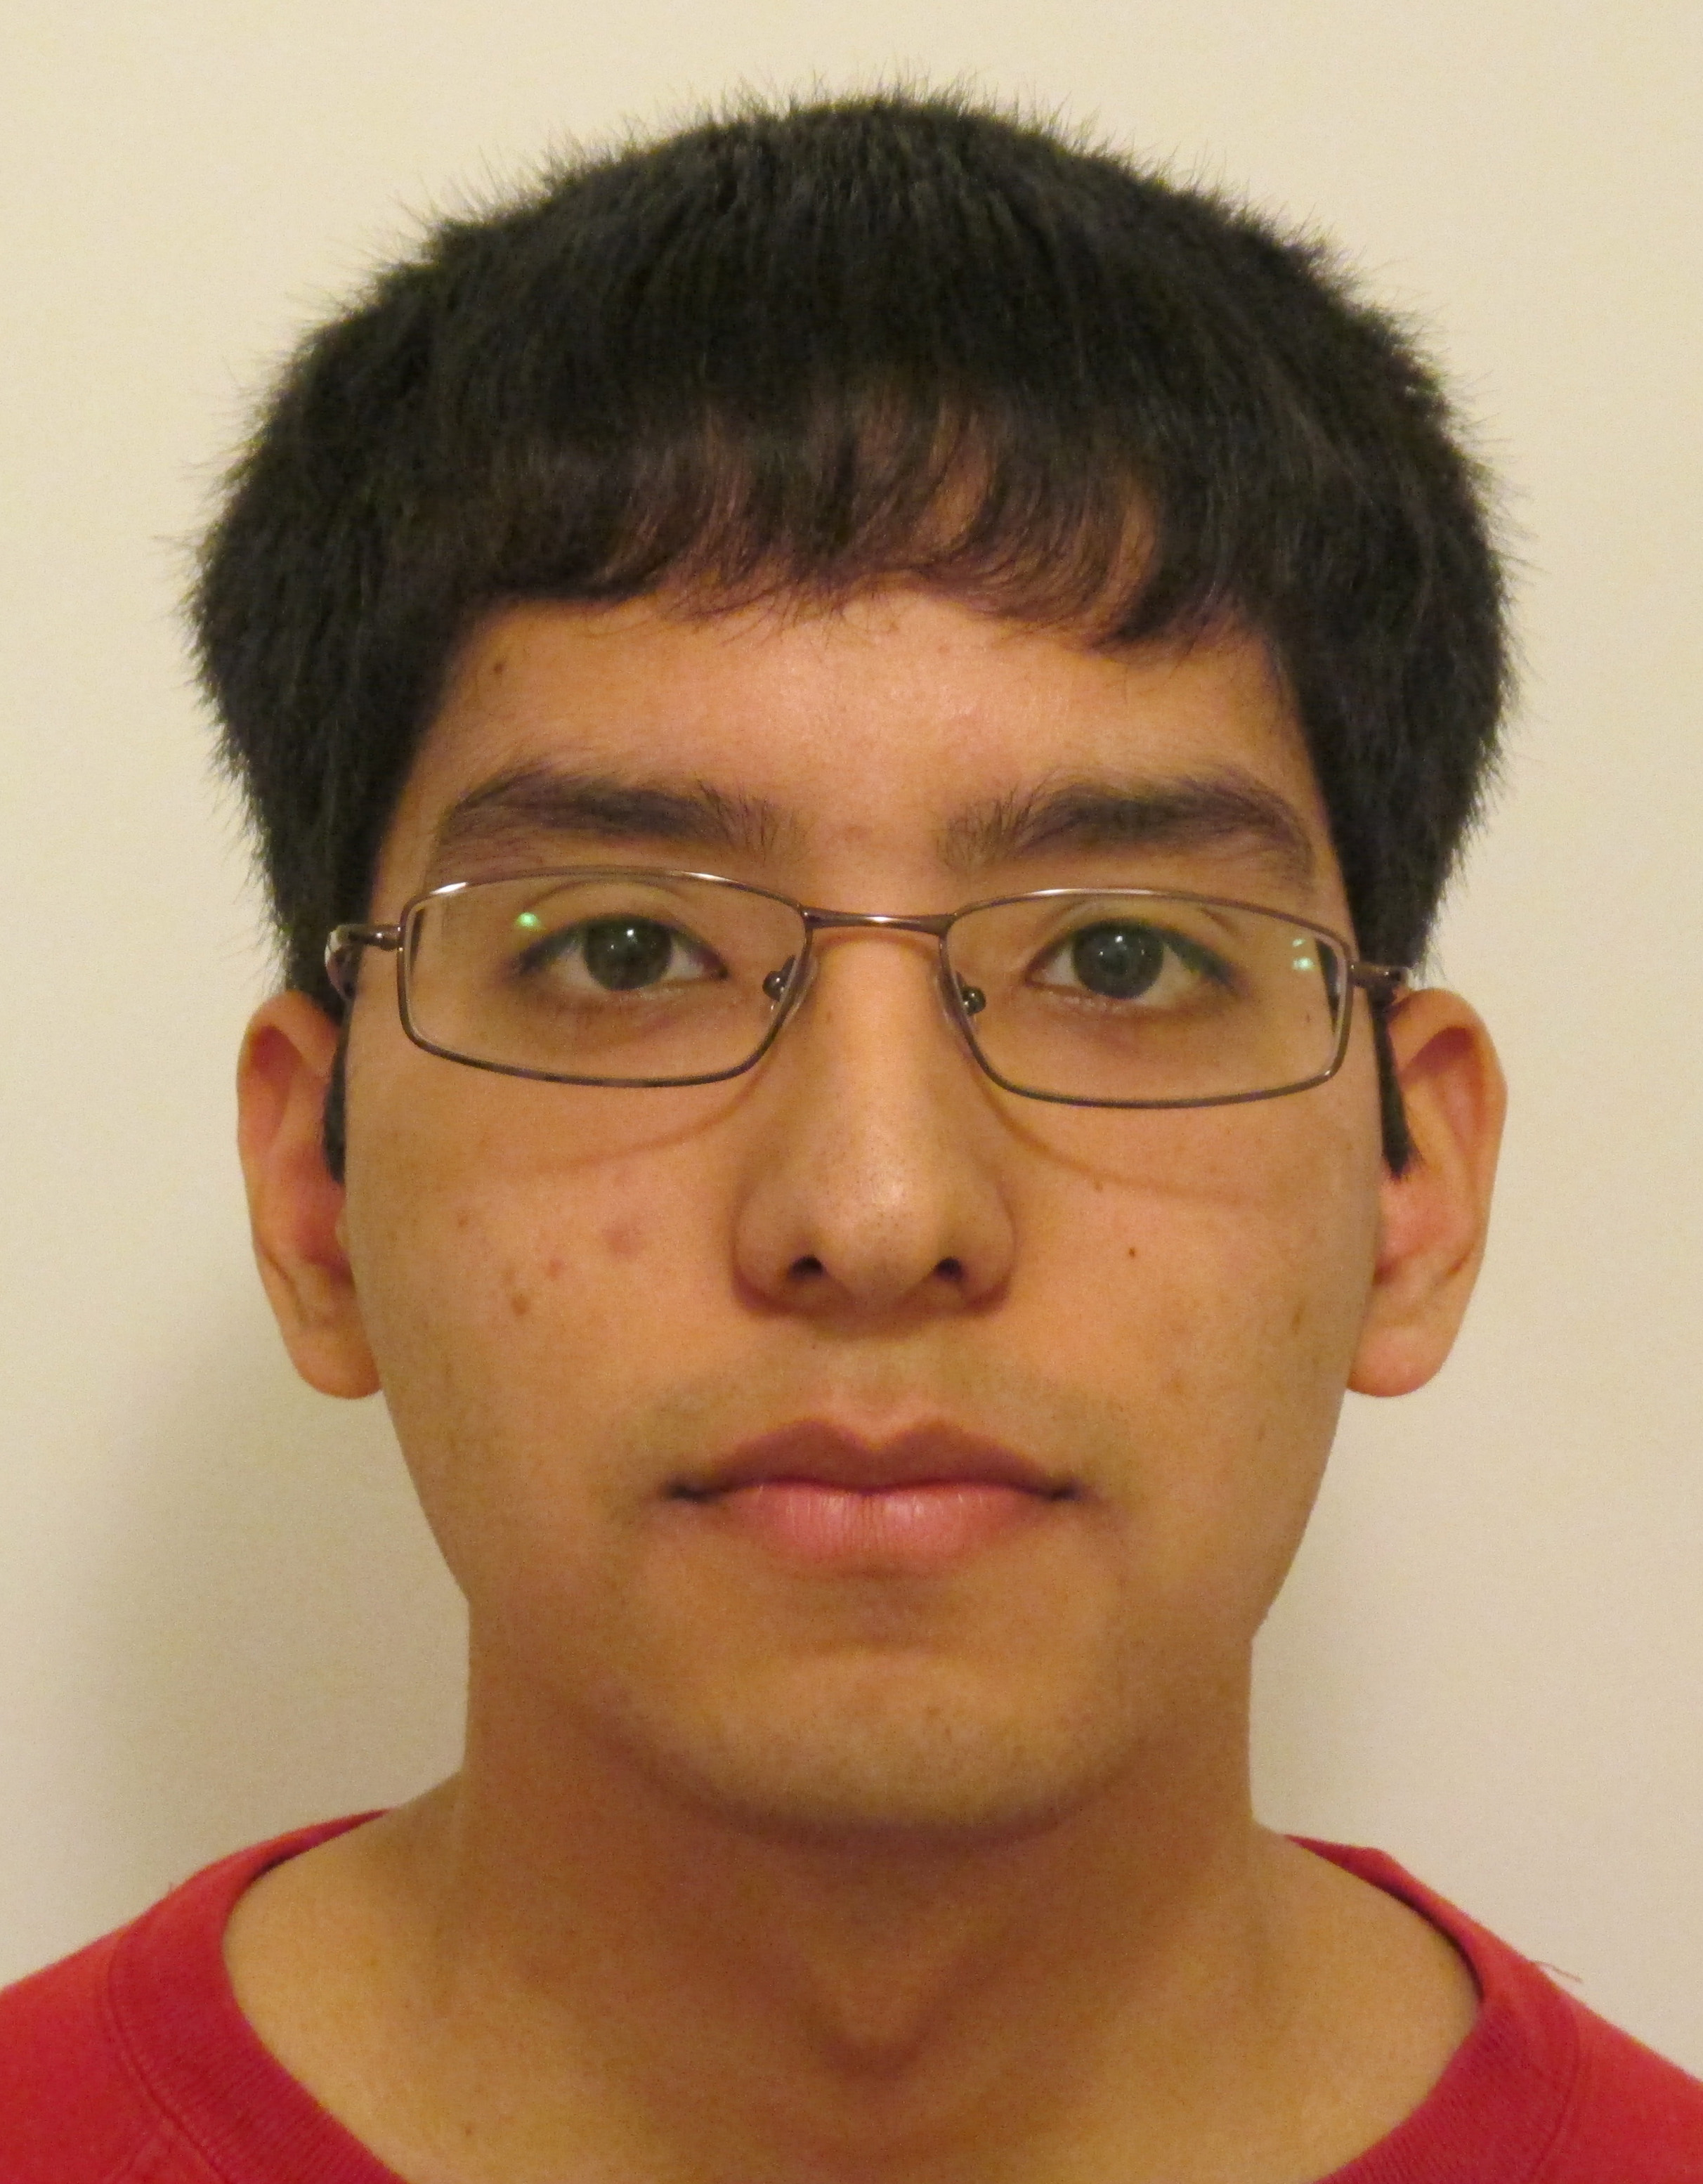
\includegraphics[height=90pt]{picture}
	\end{textblock}
\end{frame}

\begin{frame}[t]{Outline}
	\vspace{4pt}
	\begin{enumerate}
		\setlength{\itemsep}{8pt}
		
		\item About Spark {\footnotesize (what I learned, what I liked)}
		\item About the data
		\item My analysis/insights
	\end{enumerate}
\end{frame}

\section{Spark}
\stepcounter{subsection}

\begin{frame}[t]{About Spark}
	\vspace{-2pt}
	\begin{center}
		
\includegraphics[height=60pt]{spark-logo}\\[-2pt]
		Spark is a platform for large-scale data analytics.
	\end{center}
	
	\pause
	\vspace{-6pt}
	\begin{itemize}
		\item Multiple languages: Scala, Python, Java
		\item Large variety of input data sources
		\item Several libraries:
			\begin{itemize}
				\item MLlib (machine learning)
				\item GraphX (graph processing)
				\item Spark Streaming (near-real-time streaming analytics)
			\end{itemize}
	\end{itemize}
\end{frame}

\begin{frame}[t]{What I liked about Spark}
	\begin{itemize}
		\item Extremely scalable, automatically\\(10000s of nodes, PBs of data)
		\pause
		\item Very fault-tolerant
			\begin{itemize}
				\item on failure, work is moved to another worker automatically -- no data loss
			\end{itemize}
		\pause
		\item Cross-platform, runs anywhere Java runs \textit{without code changes}
		\pause
		\item Interactive shell
			\begin{itemize}
				\item can easily explore data `live', no need to compile and wait
			\end{itemize}
	\end{itemize}
\end{frame}

\begin{frame}[t]{Spark on z/OS}
	\begin{columns}
		\begin{column}[T]{0.45\textwidth}
			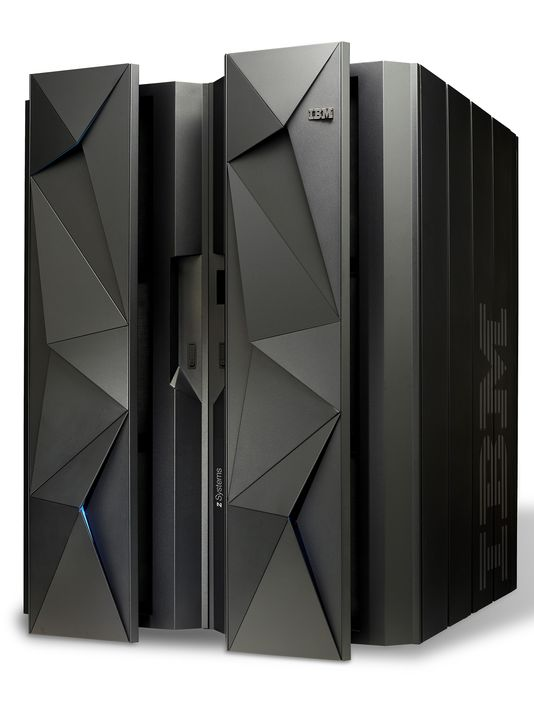
\includegraphics[width=\linewidth]{z13}
		\end{column}
		\begin{column}[T]{0.6\textwidth}
			\addtolength{\leftmargini}{-10pt}
			\begin{itemize}
				\item Run analytics right where the data is
					\begin{itemize}
						\item less network use, lower latency, security, etc.
					\end{itemize}
				\pause
				\item Can use many z/OS-native data sources
					\begin{itemize}
						\item DB2, VSAM, IMS, PDSE, etc.
					\end{itemize}
			\end{itemize}
			
			\pause
			\begin{block}{Contest system}
				z13 running z/OS, data stored in DB2
			\end{block}
		\end{column}
	\end{columns}
\end{frame}

\section{The Data}
\stepcounter{subsection}

\begin{frame}{Dataset}
	\begin{center}
		\begin{tikzpicture}[every node/.style={inner sep=0,outer sep=0}]
			\node [label={[label distance=8pt]below:{\midtilde 6000 clients}}] 
				(1) at (0, 0) {
\includegraphics[height=100pt]{people}};
			\node [label={[align=center, label distance=8pt]below:{\midtilde 1.5M transactions\\ (year 2013, \midtilde \$75.2M total)}}] 
				(2) at (5.8, 0) {
\includegraphics[height=100pt]{transaction}};
		\end{tikzpicture}
	\end{center}
\end{frame}

\begin{frame}{Clients}
	\hspace{6pt}
	\begin{tikzpicture}[every node/.style={inner sep=0,outer sep=0}]
		\node [label={[label distance=6pt]below:{\footnotesize Gender (A/B)}}] 
			(1) at (0, 3.5) {
\includegraphics[height=60pt]{gender}};
		\node [label={[label distance=6pt]below:{\footnotesize Age}}] 
			(2) at (4, 3.5) {
\includegraphics[height=60pt]{age}};
		\node [label={[label distance=6pt]below:{\footnotesize Annual income}}] 
			(3) at (8, 3.5) {
\includegraphics[height=60pt]{money}};
		
		\node [label={[label distance=6pt]below:{\footnotesize Education level}}] 
			(5) at (2, 0) {
\includegraphics[height=60pt]{education}};
		\node [label={[label distance=6pt]below:{\footnotesize Service discontinued}}] 
			(7) at (6, 0) {
\includegraphics[height=60pt]{cancel}};
	\end{tikzpicture}
\end{frame}

\begin{frame}{Transactions}
	\hspace{3pt}
	\begin{tikzpicture}[every node/.style={inner sep=0,outer sep=0}]
		\node [label={[label distance=6pt]below:{\footnotesize Client}}] 
			(1) at (0, 3.5) {
\includegraphics[height=60pt]{person}};
		\node [label={[label distance=6pt]below:{\footnotesize Date and Time}}] 
			(2) at (4, 3.5) {
\includegraphics[height=60pt]{timestamp}};
		\node [label={[label distance=6pt]below:{\footnotesize Amount}}] 
			(3) at (8, 3.5) {
\includegraphics[height=60pt]{dollarsign}};
		
		\node [label={[label distance=6pt]below:{\footnotesize Merchant name/category}}] 
			(4) at (2, 0) {
\includegraphics[height=60pt]{merchant}};
		\node [label={[label distance=6pt]below:{\footnotesize Card type/brand}}] 
			(5) at (6, 0) {
\includegraphics[height=60pt]{paymentcard}};
	\end{tikzpicture}
\end{frame}

\section{Analysis}
\stepcounter{subsection}

\begin{frame}[t]{About the Analysis}
	\vspace{6pt}
	\textbf{Predictive analytics drives smart business decisions}
	\begin{itemize}
		\item What actionable business insights can we draw from the data, using Spark?
	\end{itemize}
\end{frame}

\stepcounter{subsection}

\begin{frame}[t]{Transaction Behaviour Over Time}
	\vspace{-4pt}
	\centerline{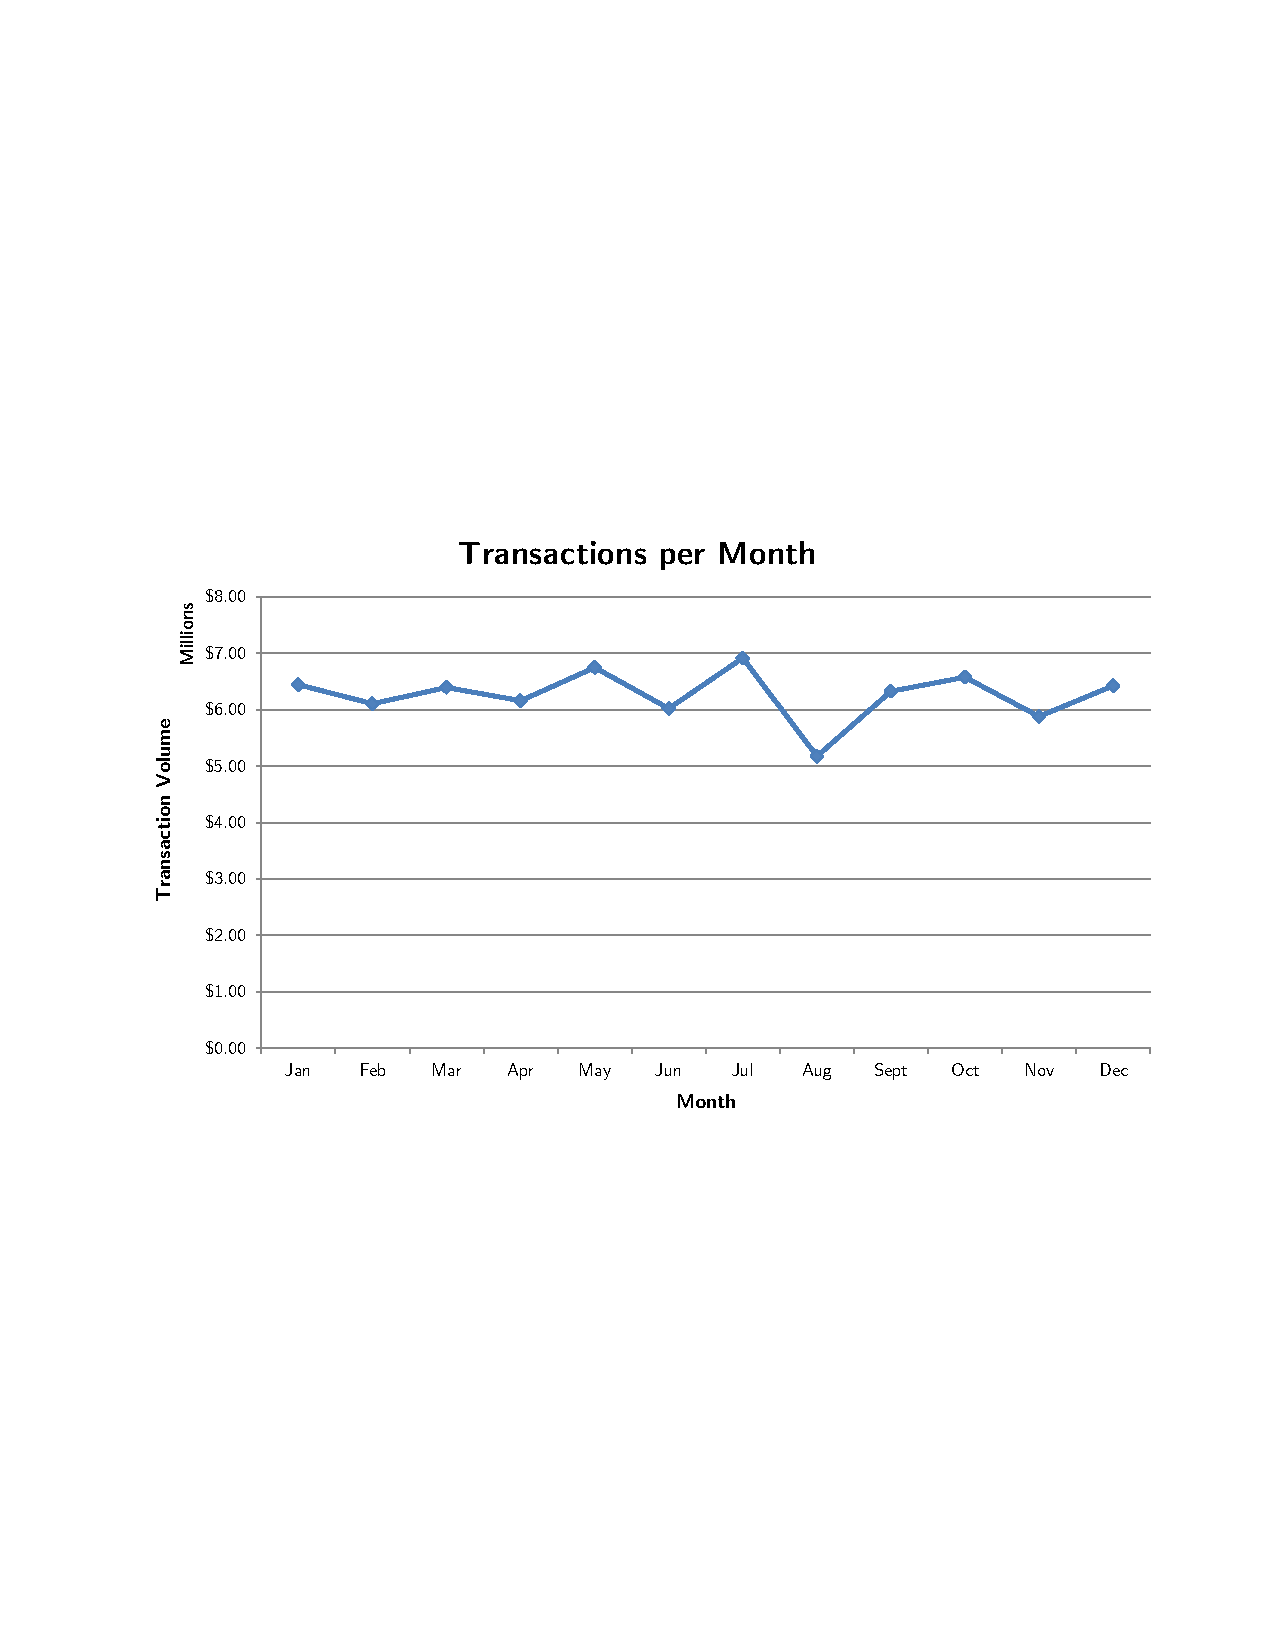
\includegraphics[width=0.9\textwidth]{transactions-per-month}}
	\vspace{-8pt}
	\begin{block}{Business Insights}
		\small
		Transaction volume is fairly steady per month.\\[-8pt]
		\begin{itemize}
			\item Probably not much benefit in monthly card promotions
		\end{itemize}
	\end{block}
\end{frame}

\begin{frame}[t]{Transaction Behaviour Over Time}
	\vspace{-4pt}
	\centerline{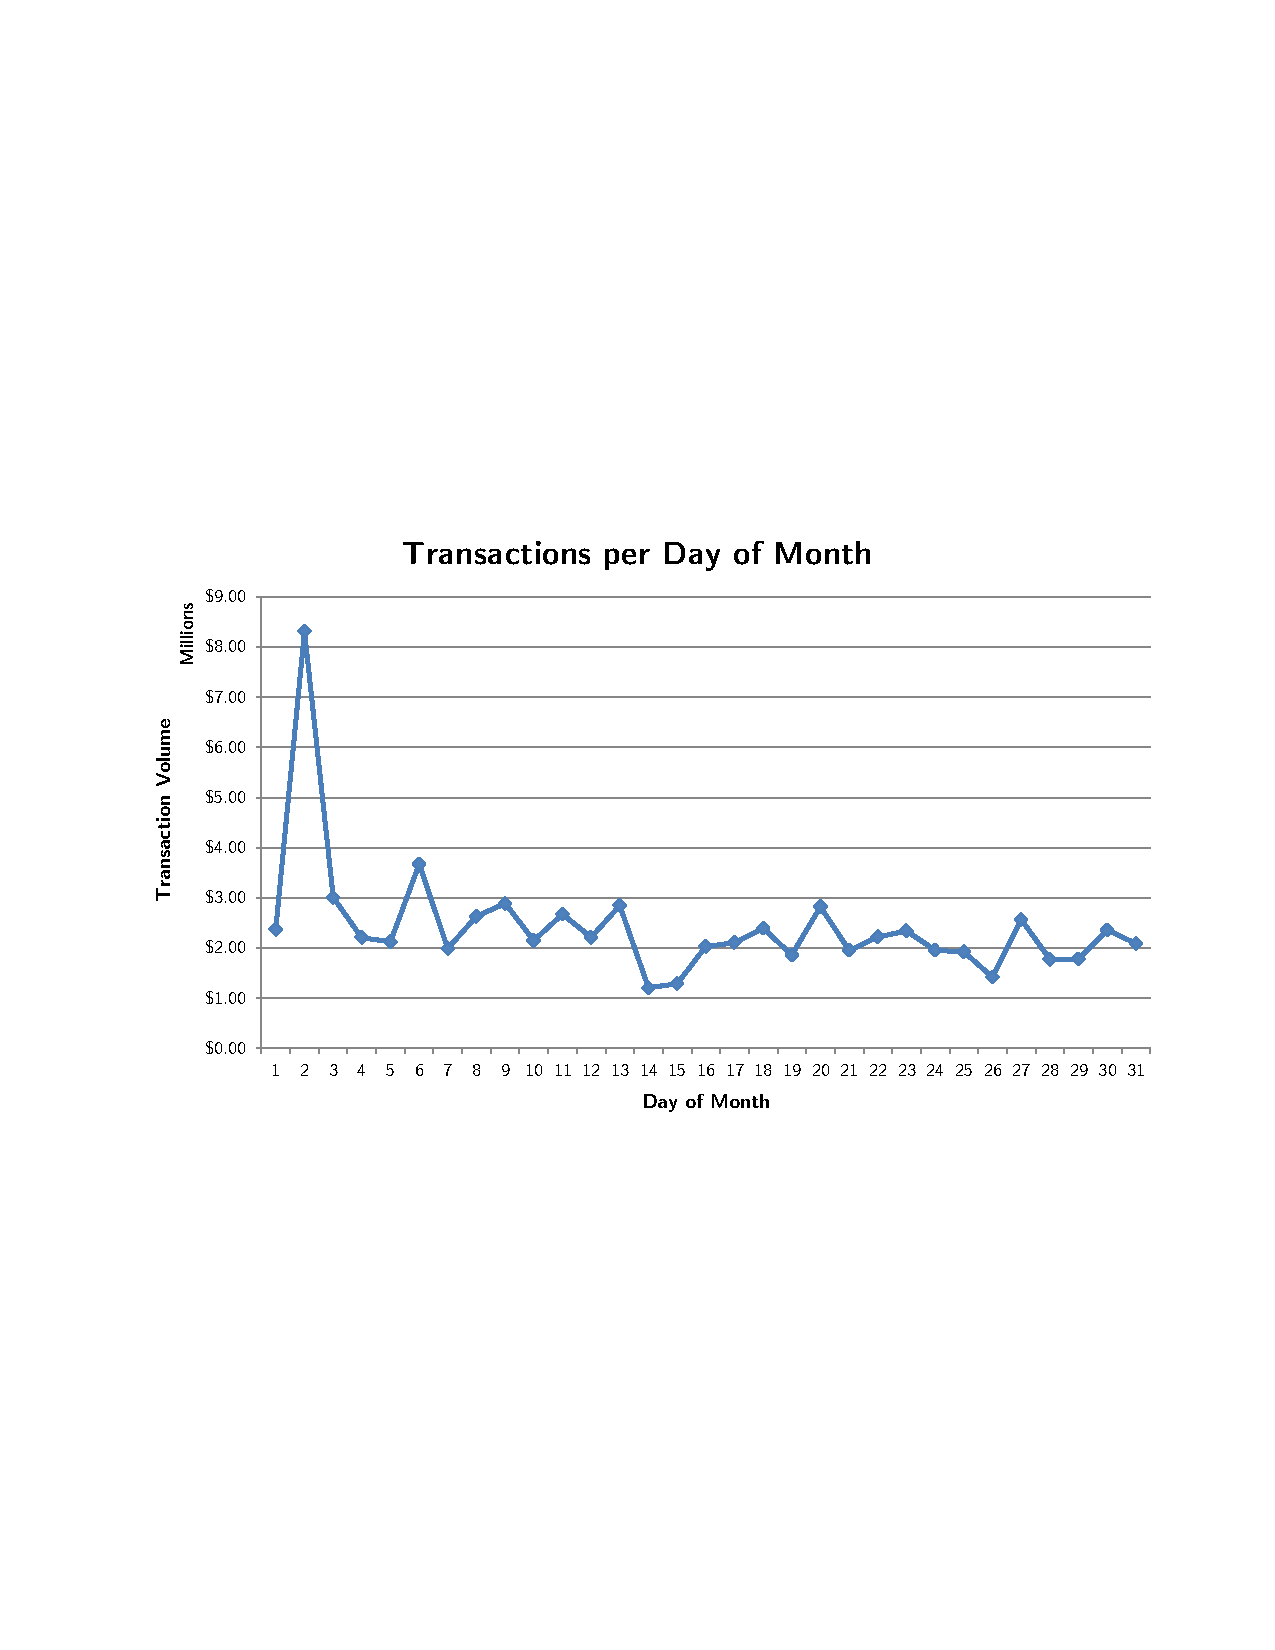
\includegraphics[width=0.85\textwidth]{transactions-per-day}}
	\vspace{-8pt}
	\begin{block}{Business Insights}
		\small
		Huge spike on the 2nd of every month.\\[-8pt]
		\begin{itemize}
			\item Businesses should be prepared for the volume and use promotions to take advantage
		\end{itemize}
	\end{block}
\end{frame}

\stepcounter{subsection}

\begin{frame}[t]{Merchant Category Insights}
	\vspace{-2pt}
	\centerline{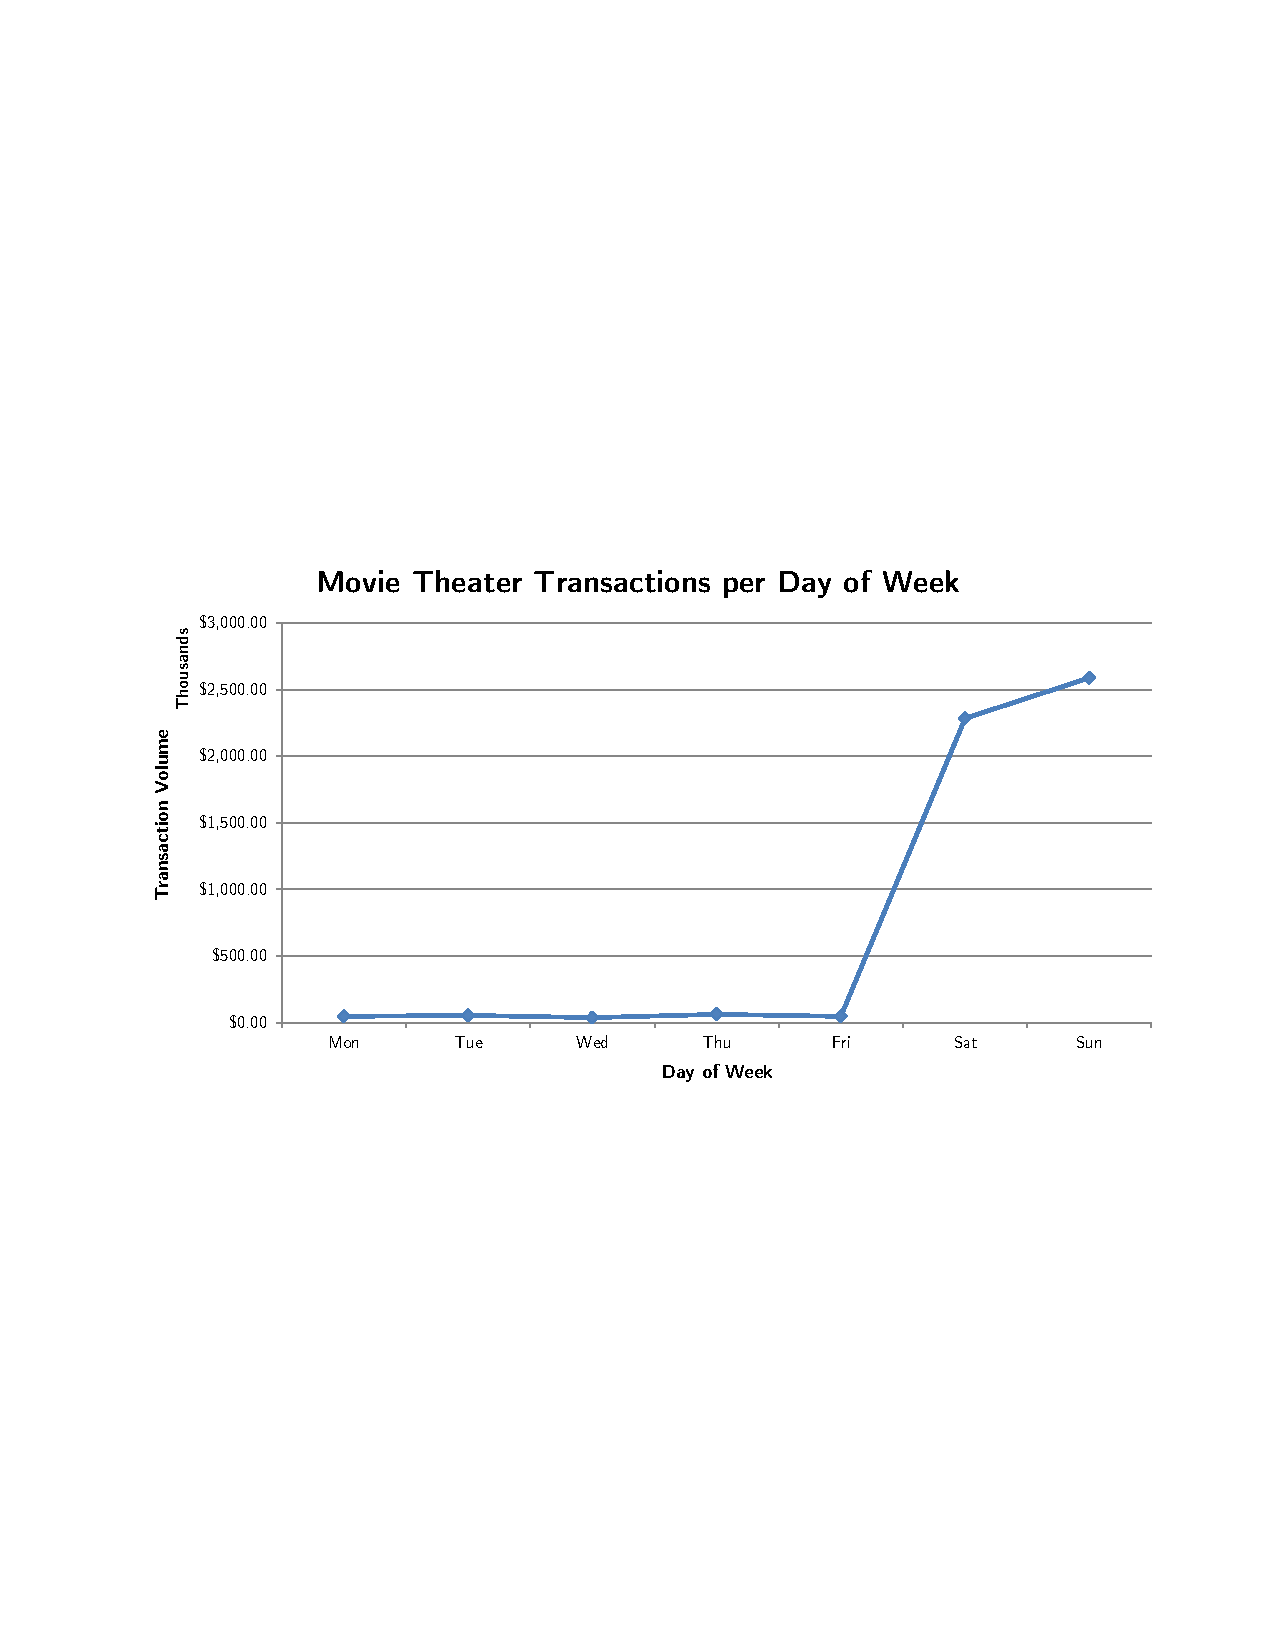
\includegraphics[width=0.95\textwidth]{movies-tx}}
	\vspace{-8pt}
	\begin{block}{Business Insights}
		\small
		\begin{itemize}
			\item Friday nights are surprisingly unpopular
			\vspace{-4pt}
			\item Weekday discounts (not just Tuesdays) could be effective
		\end{itemize}
	\end{block}
\end{frame}

\begin{frame}[t]{Merchant Category Insights}
	\vspace{-4pt}
	\centerline{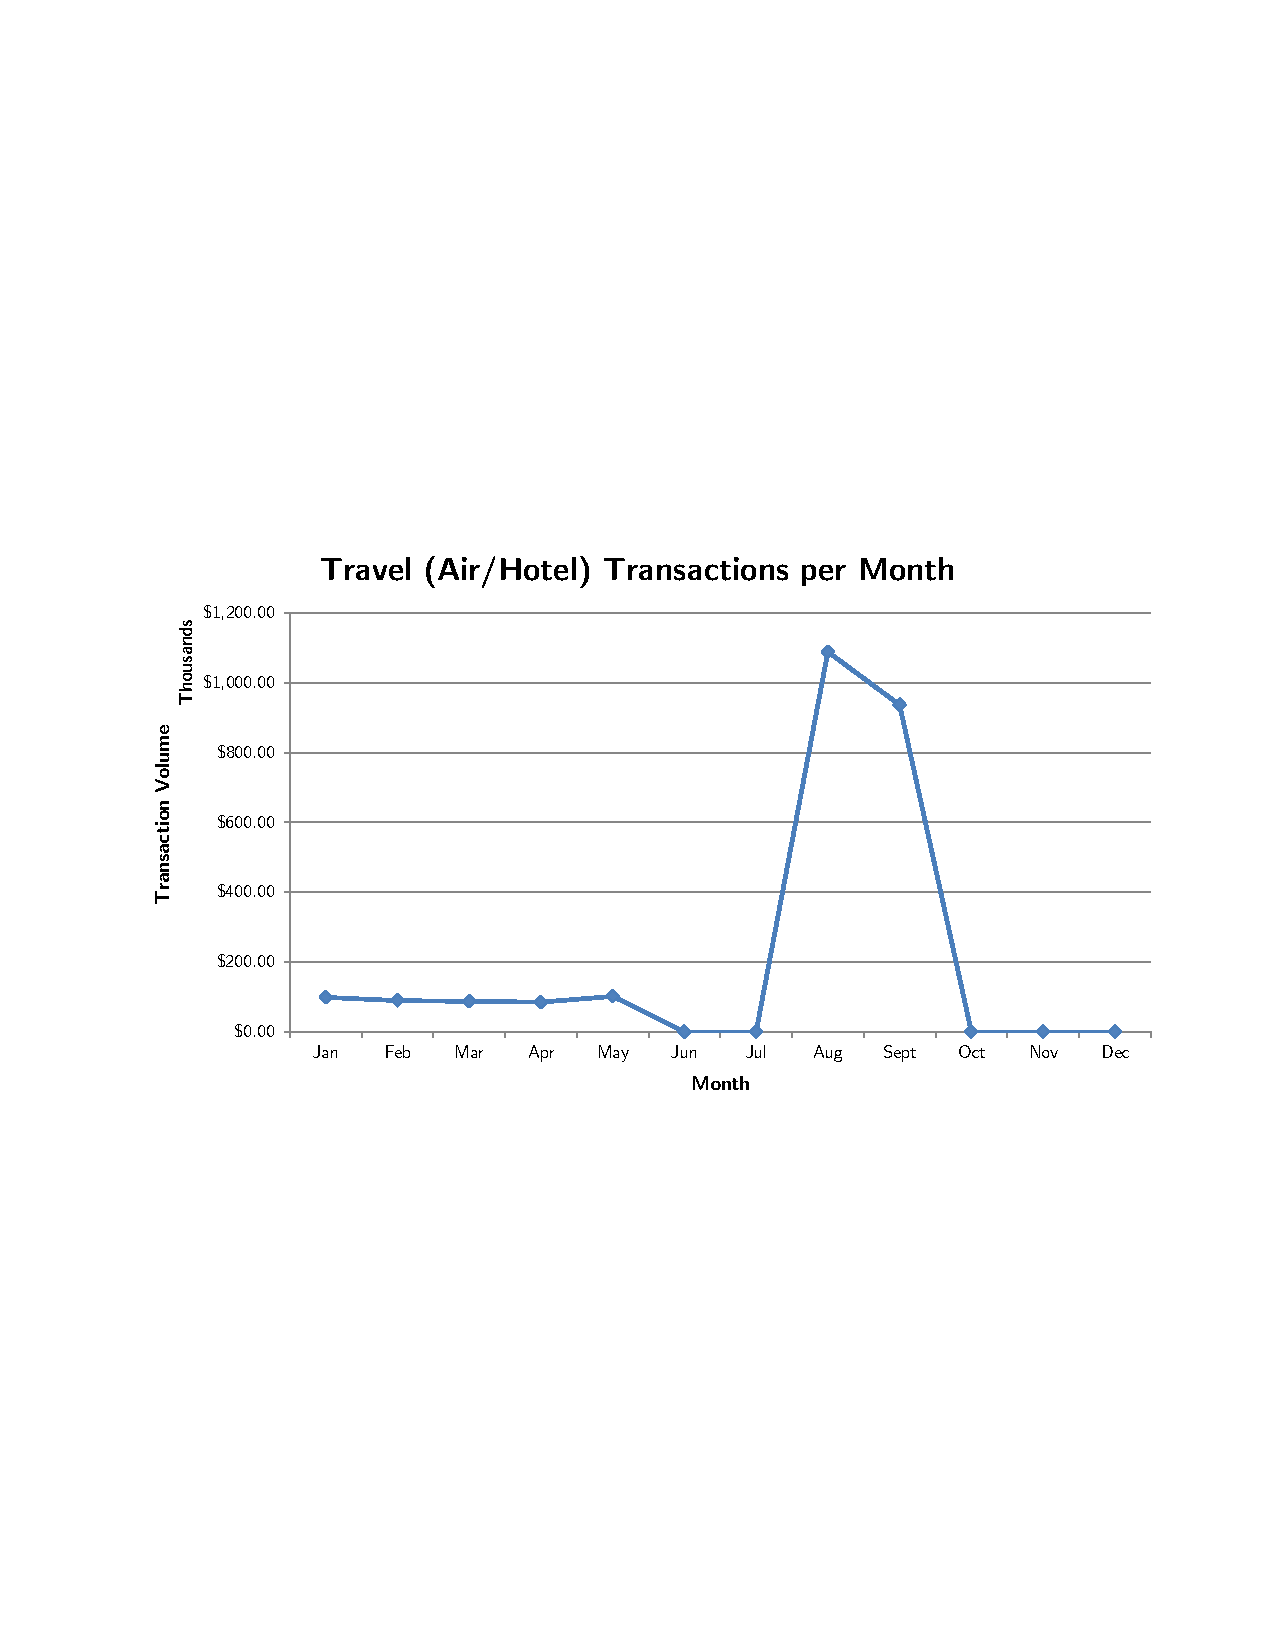
\includegraphics[width=0.95\textwidth]{travel-tx}}
	\vspace{-8pt}
	\begin{block}{Business Insights}
		\small
		\addtolength{\leftmargini}{-10pt}
		\begin{itemize}
			\item \hspace{-6pt} Travel-related businesses should anticipate the spike in Aug/Sept
			\vspace{-4pt}
			\item \hspace{-6pt} Could offer discounts in Jul/July, Oct/Nov/Dec to encourage spending
		\end{itemize}
	\end{block}
\end{frame}

\begin{frame}[t]{Merchant Category Insights}
	\vspace{-6pt}
	\centerline{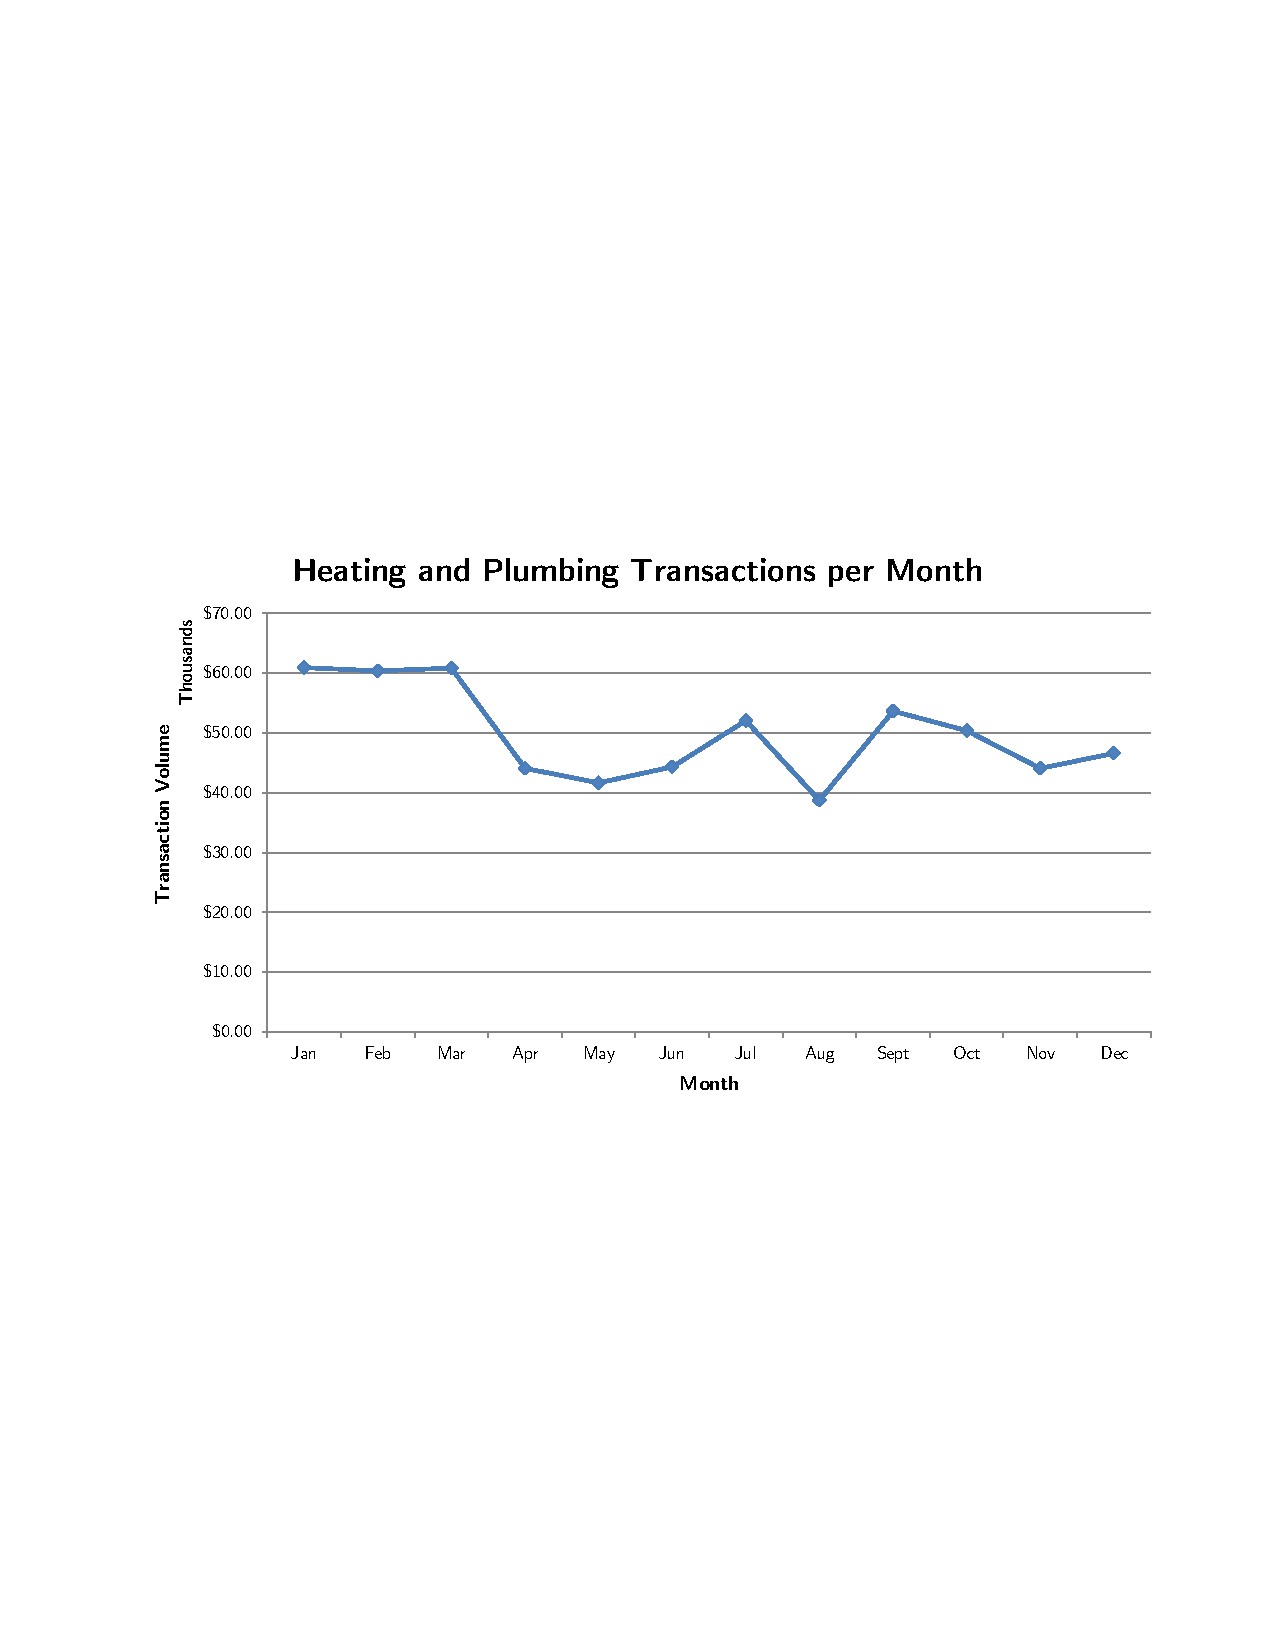
\includegraphics[width=0.95\textwidth]{heating-plumbing-tx}}
	\vspace{-8pt}
	\begin{block}{Business Insights}
		\small
		Definite monthly trends, perhaps caused by weather/climate.\\[-8pt]
		\begin{itemize}
			\item Could consider discounts in off periods, hire seasonal employees during high demand
		\end{itemize}
	\end{block}
\end{frame}

\stepcounter{subsection}

\begin{frame}[t]{Card Brands}
	\vspace{-6pt}
	\centerline{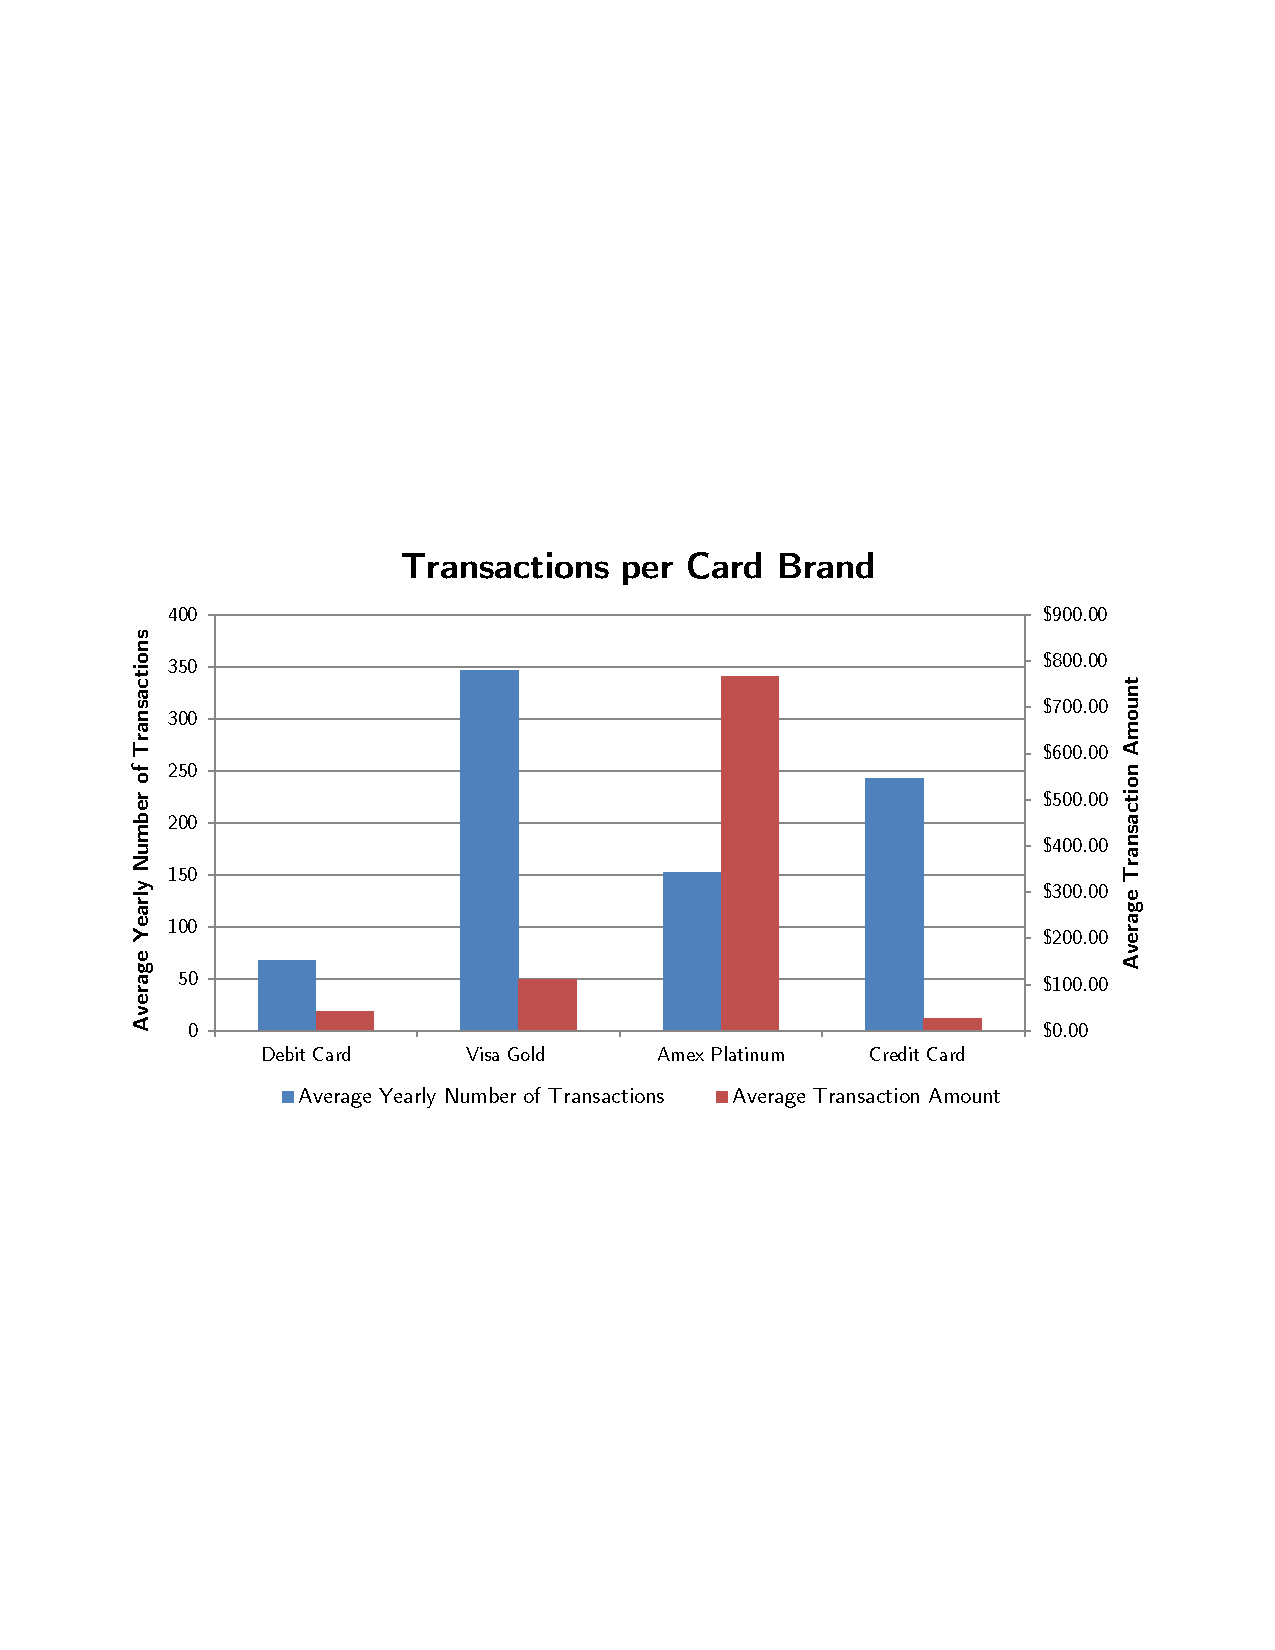
\includegraphics[width=0.9\textwidth]{brand-transactions}}
	\vspace{-8pt}
	\begin{block}{Business Insights}
		\footnotesize
		\begin{itemize}
			\item Banks should push credit cards, since people make more transactions with them
			\vspace{-4pt}
			\item Platinum card customers make much larger transactions, could push more expensive promos
		\end{itemize}
	\end{block}
\end{frame}

\stepcounter{subsection}

\begin{frame}[t]{Gender}
	\vspace{-6pt}
	\centerline{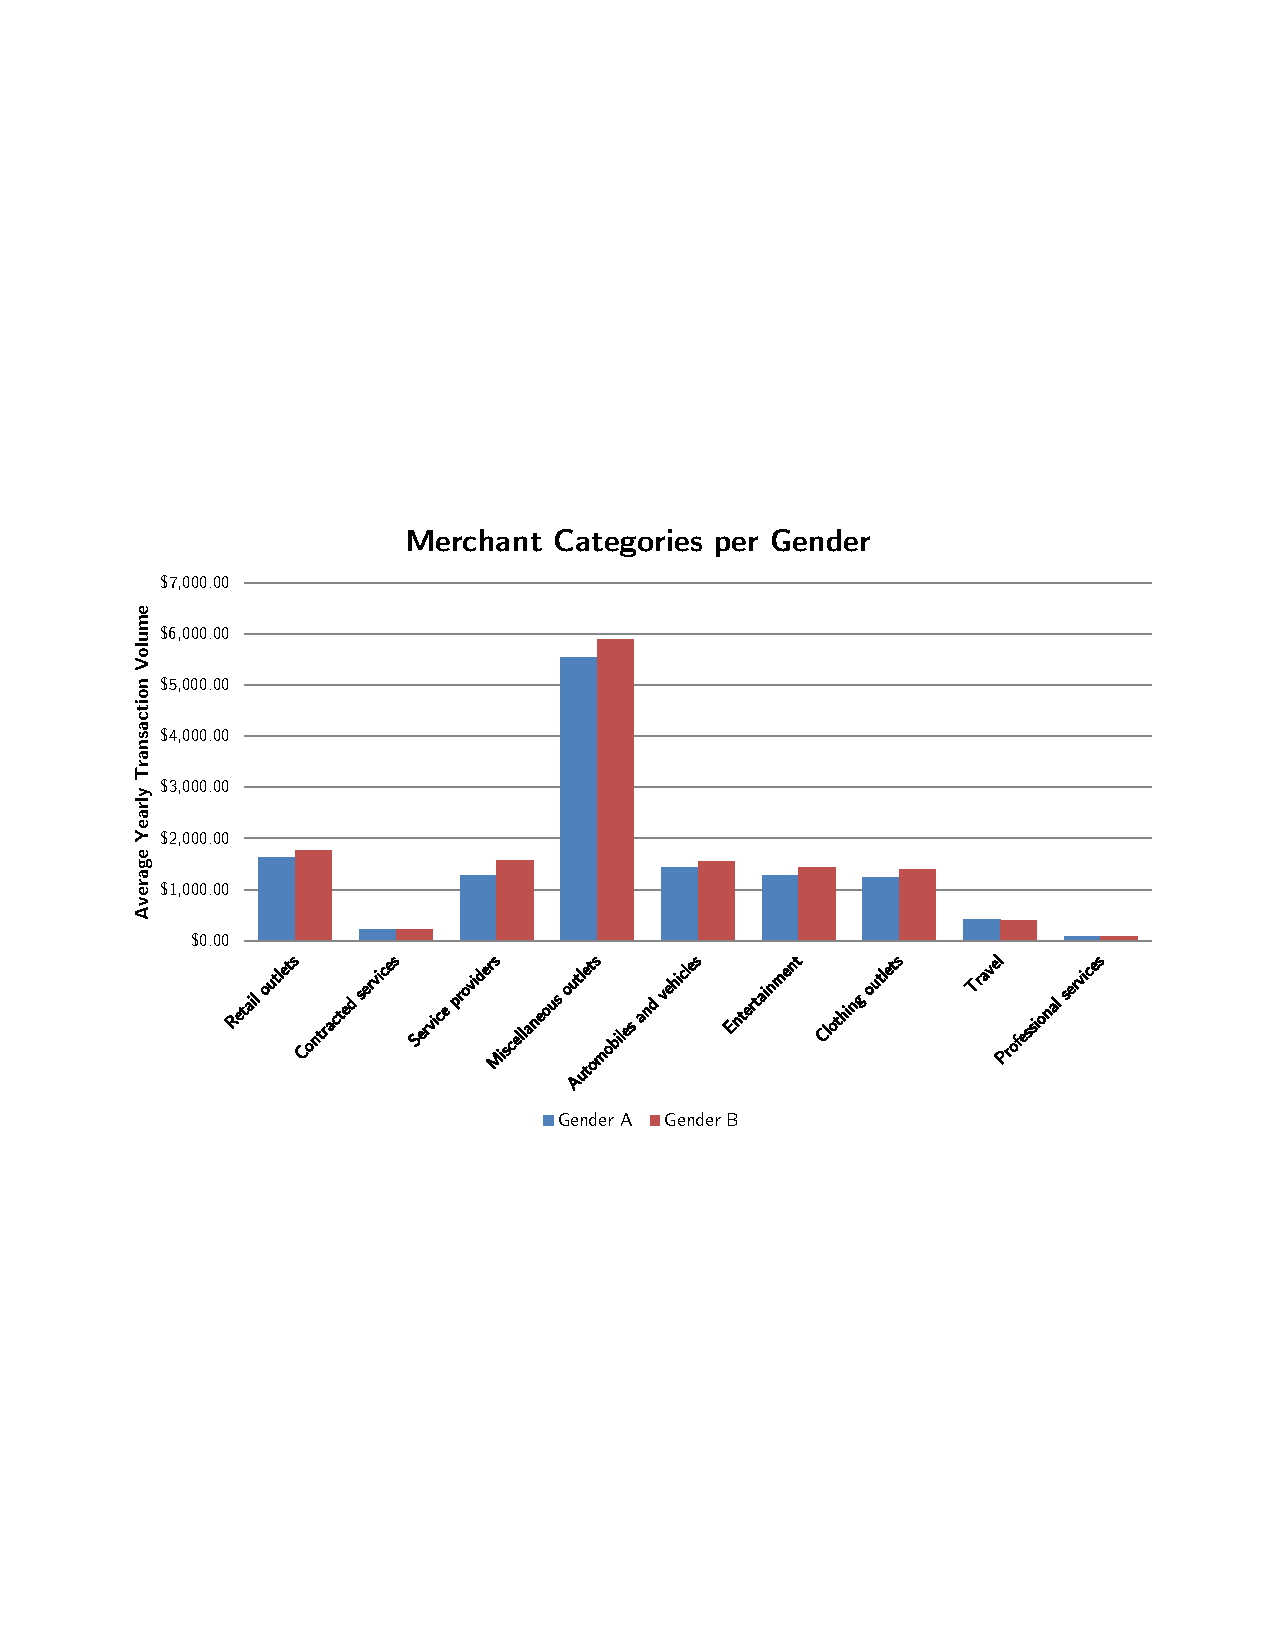
\includegraphics[width=0.95\textwidth]{cats-per-gender}}
	\vspace{-8pt}
	\begin{block}{Business Insights}
		\small
		Different genders do not seem to have different spending patterns.\\[-8pt]
		\begin{itemize}
			\item Gender-specific marketing may not be so effective
		\end{itemize}
	\end{block}
\end{frame}

\begin{frame}[t]{Age}
\vspace{-2pt}
	\centerline{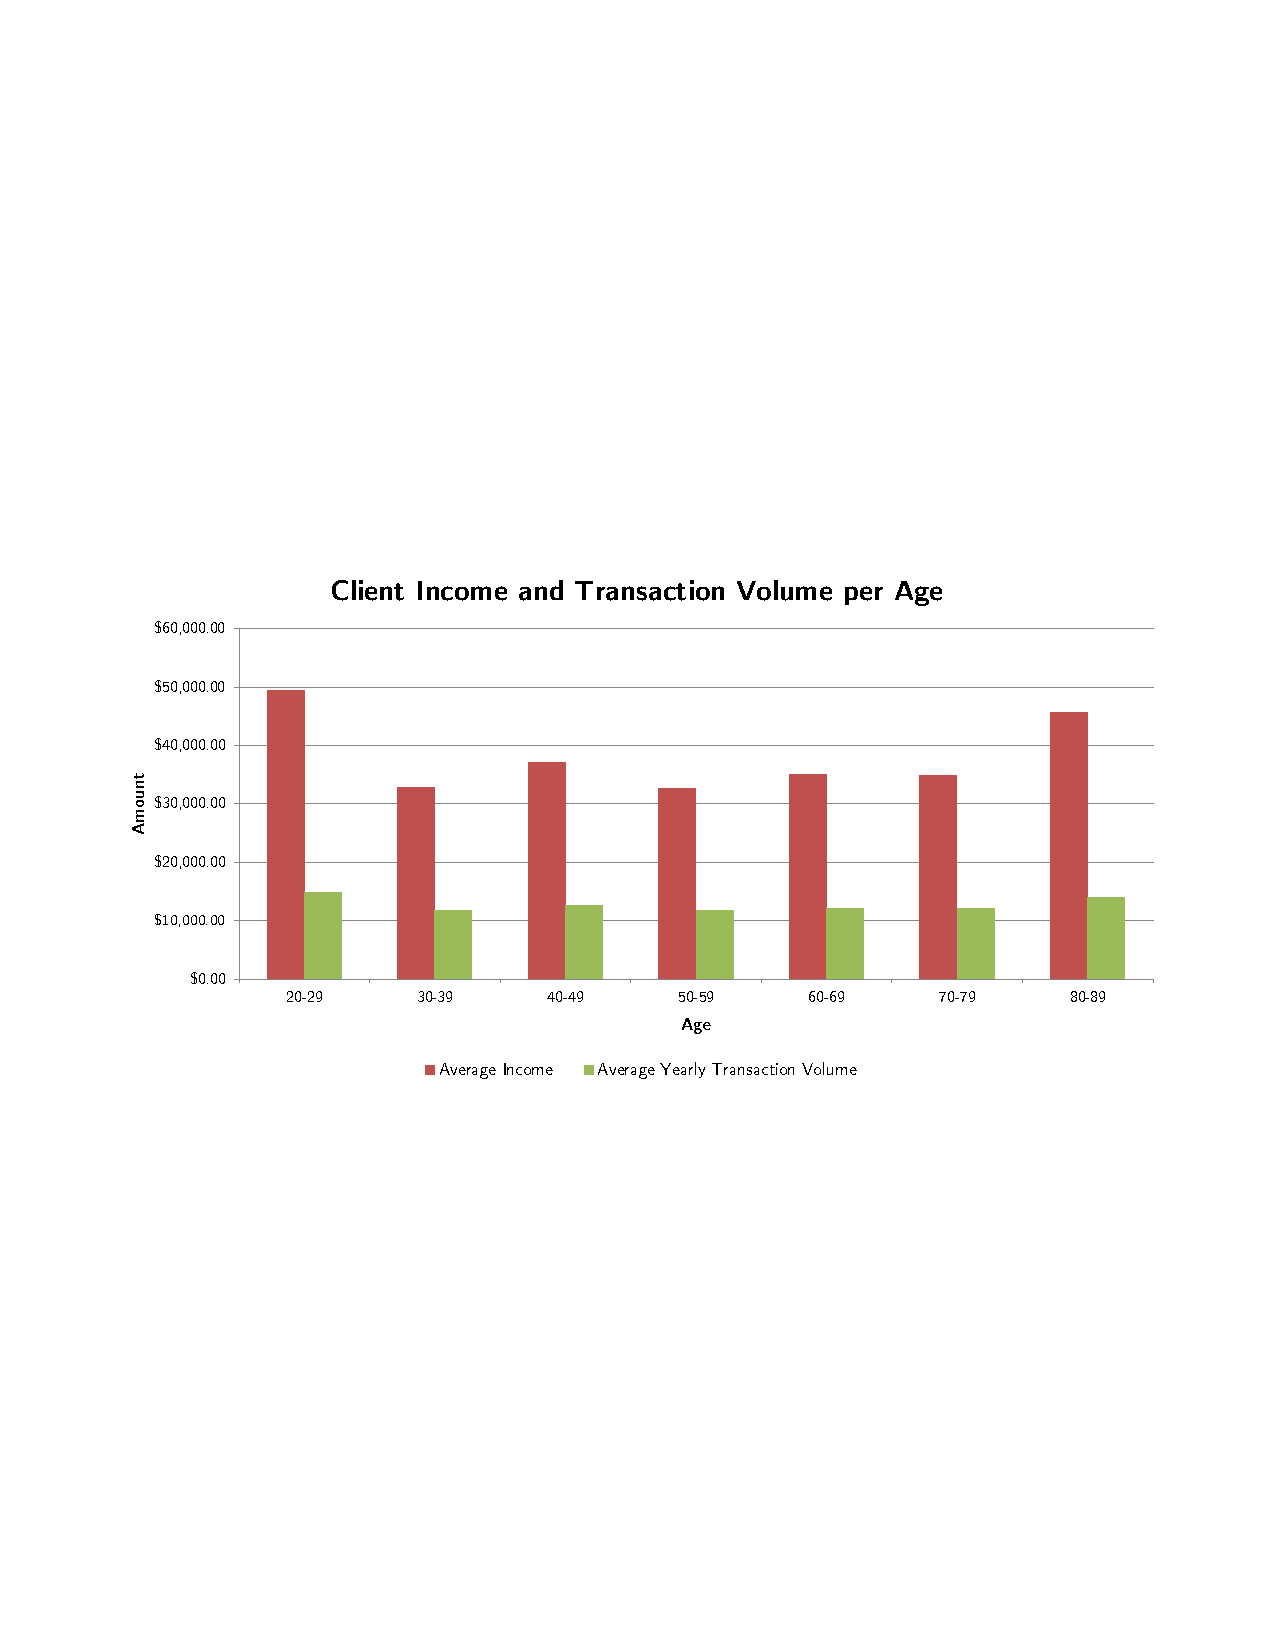
\includegraphics[width=1.05\textwidth]{age-money}}
	\vspace{-6pt}
	\begin{block}{Business Insights}
		\small
		Young and old clients have more income, but do not spend more money.\\[-8pt]
		\begin{itemize}
			\item Age-specific marketing may not be so effective
		\end{itemize}
	\end{block}
\end{frame}

\setcounter{section}{0}
\setcounter{subsection}{0}

\begin{frame}[t]{}
	\begin{center}
		\begin{exampleblock}{}
			{\large ``Information is the oil of the 21st century, and analytics is the combustion engine.''}
			
			\hspace*\fill{\small--- Peter Sondergaard, Gartner Research}
		\end{exampleblock}
		
		\vspace{12pt}
		\textbf{Thanks! Questions?}
		
		\vspace{8pt}
		\begin{center}
			\begin{tikzpicture}[every node/.style={inner sep=0,outer sep=0}]
				\node [label={[label distance=6pt]below:{\footnotesize Me: Stephen Solis-Reyes}}] 
					(1) at (0, 0) {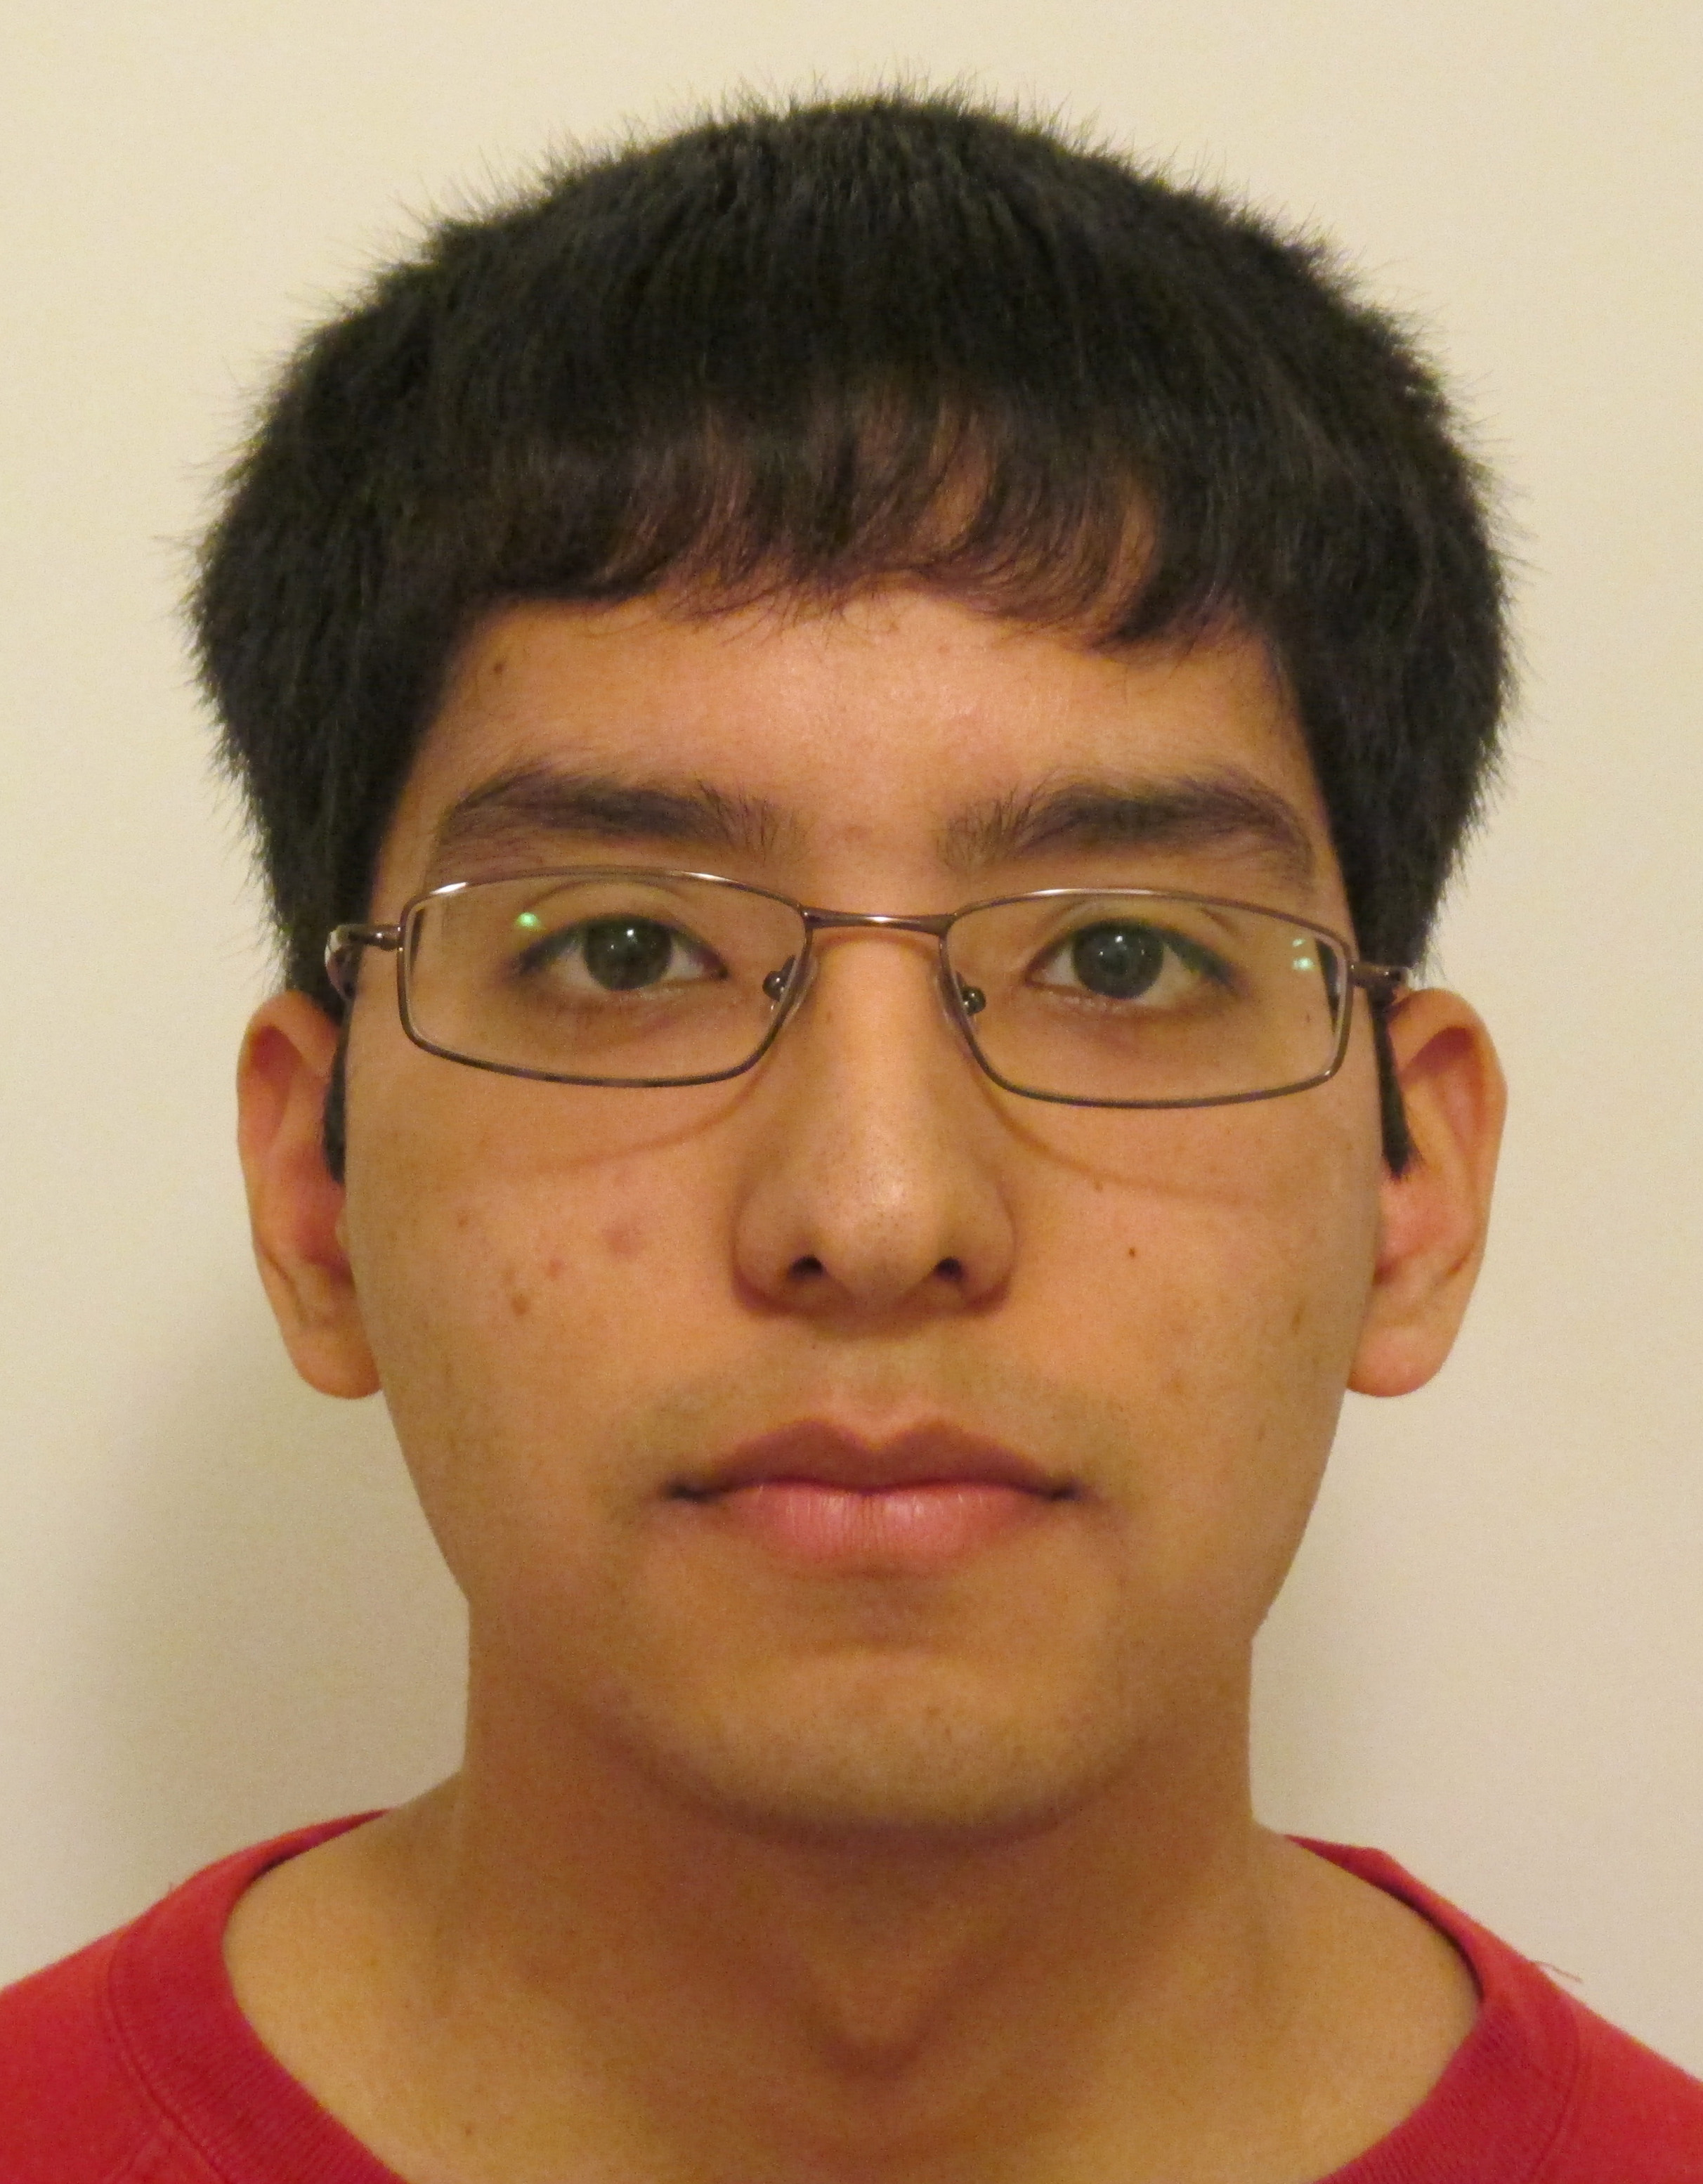
\includegraphics[height=90pt]{picture}};
			\end{tikzpicture}
		\end{center}
	\end{center}
\end{frame}

\end{document}
